\subsection{Survey method} \label{sec:survey}

In this section we depict the methodology we followed to collect papers related to traceability with a peculiar scrutiny on works aiming at modeling/representing traceability information and purposes.


%\subsection{Publication selection process}
\begin{figure}[h]
	\centering
	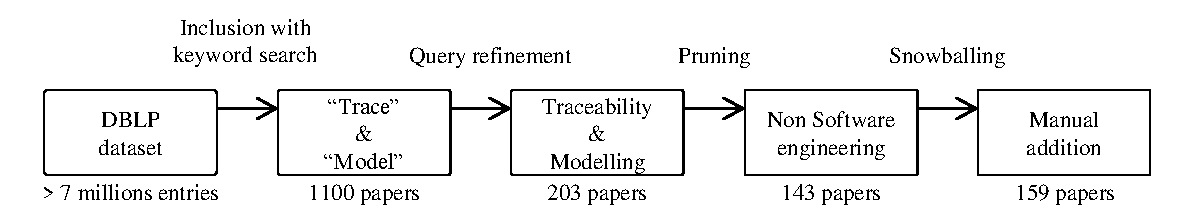
\includegraphics[width=.9\linewidth]{images/survey-process}
	\caption{Process of the survey on traceability and modeling. }
	\label{fig:surveyprocess}
\end{figure}
%\begin{figure}[h]
%	\centering
%	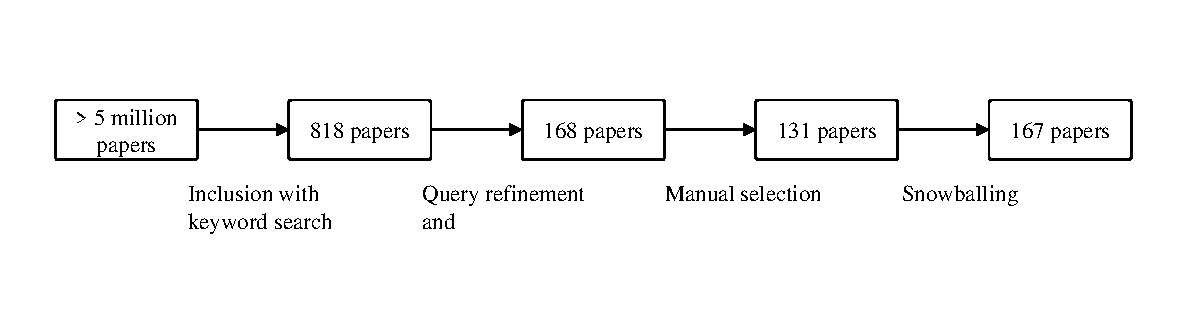
\includegraphics[width=.9\linewidth]{images/survey-process2}
%	\caption{process of the survey on traceability and modelling. }
%	\label{fig:surveyprocess}
%\end{figure}
The approach selection process was conducted in three main steps illustrated in \Fig{fig:surveyprocess}. First, we started selecting approaches based on our own experience about working on traceability during the last past years together with recent meta-studies on the topic, \textit{e.g.,}~\cite{Gotel2012,antoniol2017-traceability-grand-challenges,clelandhuang2014-traceability-trends-and-futurte-direction,guo2017-semantically-enhanced-tracebility-deep-learning}. This very first selection contained a dozen distinct studies we were personally aware of.  

Then, to complement our knowledge and explore the maximum of published work on traceability, we decided to mine bibliographic data sources following the literature review process established by Kitchenham and Charters~\cite{kitchenham2008}.
Finally, we pruned the resulting selection to remove papers not related to our topic.


\subsubsection{Data source and search strategy}
We used DBLP (2020-07-01~\cite{dblp}) as our core electronic database to search for primary studies on traceability.
To avoid missing possibly relevant approaches, we decided not to put a specific period constraint for the search, but we limited the scope of the search to paper of five pages or more to avoid posters, tool demos and other types of short papers.
Based on the topic of this survey, we defined the terms of the search query according to the recommendations of Kitchenham and Charters~\cite{kitchenham2008}. 
As we are looking for papers proposing traceability techniques for software engineering we first considered the terms "trace" and "tracing" together with the seminal spelling "model" referring to modeling, as well as model-based variations. The idea of this first attempt was to include as many proposals as possible by using these generic model-based terms that should be part of any traceability work (as both, traces must be represented, typically as some kind of model, and many traceability approaches use models as source or target of the traces).

Nevertheless, this resulted in too large a number of results with 1100 papers matching the query. Potential papers, at first sight, consisted in a vast majority of false positives. Indeed, "Model" is used in too many fields, "traces" as well, and papers related to software engineering were scarce.
%Since we are not necessarily interested in publications figuring concrete applications of traceability but rather modelling (in a broad sens) work on traceability, we narrowed the scrutiny of the search to work on traceability (modelling tracing) only and we refined once more our query with "traceability", "traces", and "tracer" instead of "trace" for a selection of 771 papers.
Therefore, we refine the query including keywords more akin to modeling and software engineering, focusing more on papers mentioning traceability and not just trace and "modeling" (and its variations and related concepts: "language", "DSL", "transformation", "MDA", "MDD"). This refinement brought down the selection of 203 papers. 

Here is the exact query we applied:
\begin{verbatim}
	.*(([Tt]rac(eability|ing))|([Tt]race[rs])).* AND
	.*(([Mm]odel[- ])(([Dd]riven)|([Bb]ased))|MD[DAE]|Model[l]ing|
	[Tt]ransformation|DSL|[Ll]anguage).*
\end{verbatim}


\subsubsection{Pruning}
In what follows (and as proposed by Kitchenham and Charters~\cite{kitchenham2008}), we describe the used inclusion and exclusion
criteria. We further explain how we applied these criteria on the previous set of papers. 

\textit{Inclusion criteria}
\begin{enumerate}
	\item the work is a software engineering approach
	\item the paper is about tracing software engineering
	\item traceability is the main concern
\end{enumerate}

\textit{Exclusion criteria}
\begin{enumerate}
	\item the paper is not a primary study
	\item paper is not a white paper
\end{enumerate}

Before we applied these criteria on the potential papers fetched by our query, we removed automatically papers of less than 5 pages long.
We then extracted automatically papers whose titles mention "biology", "education", "kinetics", "logistics", "physiology", "physics", "neuroscience", "agriculture", and "food" which seem to appear each in a couple of selected papers. This helped in the application of the exclusion criteria. We manually examined the 183 papers left and excluded 60 papers that did not fulfilled the criteria or were duplicates.
% for a remaining total of 123.

\subsubsection{Snowballing}
Following the application of our methodology, we wanted to double-check that we did not miss any potentially relevant approach. Indeed, some papers could have been missed during the search process for different reasons. For instance, some workshop papers are only indexed by ACM and some other papers have not yet been indexed by DBLP. Furthermore, some papers are not actually using the term "trace" or similar in the title (e.g., if they present so-called composition or extension approaches sometimes used as traceability mechanism). Finally, we added papers we found following the selected papers references and added papers from a specific event on traceability, the ECMFA workshop on traceability (\ie ECMFA-TW). The final result of the overall process (including this last snowballing phase) presented 159 papers. Among them, there are 41 articles, 82 in proceedings, and 36 workshop reports (see Table \ref{tab:classification-tm}).
\Fig{fig:publicationyears-tm} shows the chronological distribution of this selection of publications.


\begin{figure}[h]
	\centering
	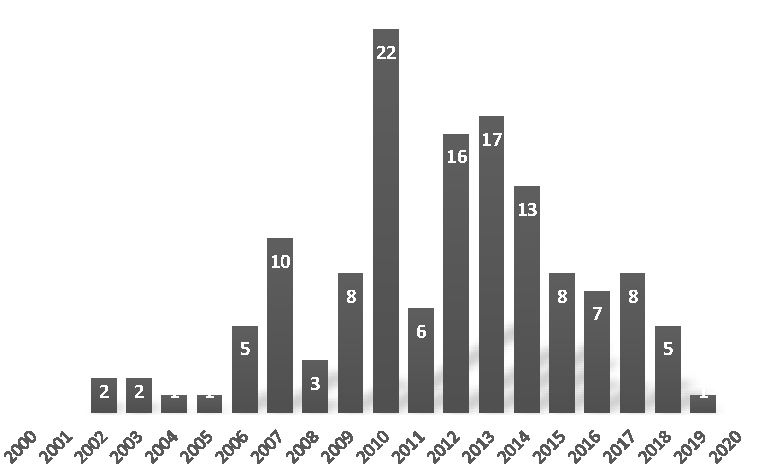
\includegraphics[width=.6\linewidth]{images/publicationyears-tm}
	\caption{Papers selected related to traceability and modeling. }
	\label{fig:publicationyears-tm}	
\end{figure}

\begin{table}[h]
\centering
	\begin{tabular}{|ll|}
		\hline
		\multicolumn{2}{|l|}{\textbf{Publication type}}  \\ \hline
		\multicolumn{1}{|l}{Journal}          & 41       \\ \hline
		\multicolumn{1}{|l}{Conference}       & 82       \\ \hline
		\multicolumn{1}{|l}{Workshop}         & 36       \\ \hline
	\end{tabular}
	\caption{Publication types of the selected papers.}
	\label{tab:classification-tm}
\end{table}



\subsubsection{Threads to validity in the selection process}
We acknowledge limitations in the execution of our survey method. 
First, we only used DBLP as a source database. Yet, it is recognized as a {representative} electronic database for scientific publications on software engineering and already contain more than five millions publications from more than two millions authors.
Setting the limit based on the number of pages alone to elude short papers is another threat to validity. Yet, it is a reproducible practice that limits the number of papers to analyse and thus helps concentrate on the topic rather than the engineering of the survey. 
Then, the vocabulary related to traceability is scattered among various fields of application with their respective nuances. We mitigate the risk of missing papers with a broad query and we remind the reader that, in this survey, we want to target papers explicitly mentioning traceability -- and doing so, working on the emergence of a search field in itself. 

%\subsection{General trends in traceability and modelling}\label{sec:trendsTM}
%The results of the survey are manifold. First, they explicit the dual nature of traceability approaches where the frontier between augmenting traceability and augmenting a software task with traceability is often very thin. 
%\ugh{(rq1)} We found that traceability is specifically adapted to model-based environment, which various levels of abstraction  allows rich representations of trace artefacts~\cite{santiago2013traceability-in-MDE}. MDE automated tasks are moreover prone to generate traces during their execution - including the execution of higher-order transformations supporting co-evolution between modelling artefacts~\cite{la_Fosse_2018}. 
%\ugh{(rq2)}Then, we found evidences of the penetrating importance of machine learning techniques to bridge the semantic gap that separates natural language document and coded elements of a software system. 
%\ugh{(rq3)}Finally, we found that traceability augments the automation potential of many tasks at every phase of the lifecycle and a raw map of the knowledge area covered by traceability approaches emerges.
%We give details on these different points in the next sub-sections.

%\textbf{Insert some \textbf{statistical distribution} (MM/Meta/concrete application | Modelling traceability vs Tracing modelling | identification of traces | Req. vs other | unstructured text vs others (code, or design model))...}
%63 papers are related to requirement traceability (tracing requirements to other software artefacts).
%8 Meta studies
%76 approaches presenting a language or a framework, and 41 explicitly describing a metamodel.
%22 approaches to trace identification with IR techniques
%22 target source code
%51 target model-level artefacts maintenance and understanding
%





